% !TEX root =  ../gesamtkonzept.tex
\subsection{Architektur}

% PLAGIAT - so aus meiner BA, wird natürlich umformuliert, erstmal nur schon drin, weil wir uns ja in ne ähnliche Richtung bewegen

% hyperref auskommentiert, weil dazu ja nix existiert. -> integration in bestehende system könnte man eventuell erwähnen, wenn man das Backend von wo anders aus auch ansteuern wollen würde unso, man muss ja net unser frontend nutzen.
Das neue System setzt auf das Client-Server-Modell, um einen mehrfachen und voneinander unabhängigen Zugriff sowie die Entwicklung von Erweiterungen zur Integration in bereits bestehende Systeme zu ermöglichen, womit Anforderung 
%\hyperref[Anf:A1]{A1}, die Umsetzung des Systems als Webanwendung, 
abgedeckt werden soll.
Dabei stellt der Server eine \ac{API} für den Client zur Verfügung, um auf alle Ressourcen zugreifen zu können.
Die Geschäftslogik befindet sich deshalb im Server, da der Client lediglich für die Darstellung verantwortlich ist.
Der Client stellt dabei die Visualisierungsmethoden zur Verfügung und arbeitet die über die Schnittstelle gesammelten Daten auf.

\begin{figure}[h]
  \centering
  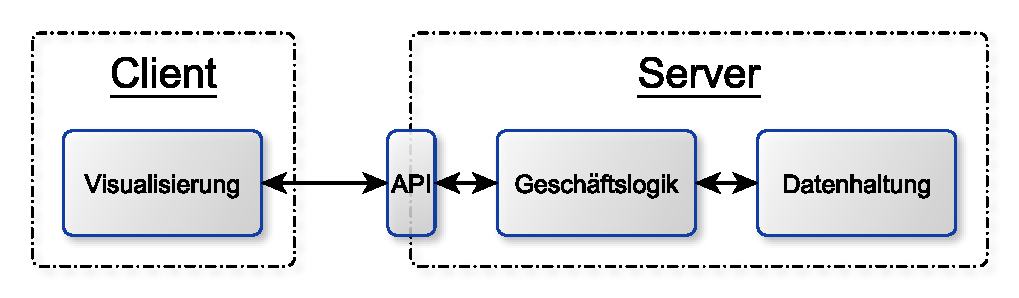
\includegraphics[width=0.75\textwidth]{img/konzeption/gesamtkonzept/Architektur.pdf}
  \captionsetup{format=hang,justification=raggedright,singlelinecheck=false}
  \caption[Architekturmodell]{Architekturmodell. \\Quelle: Eigene Darstellung.}
  \label{img:einkaufBPMN}
\end{figure}

Grundlegend ist die Architektur somit dem \ac{MVC}-Konzept nachempfunden, so stellt der Server das Model durch die vorhandene Datenbank und die darin vorhandenen Relationen.
Der Controller wird zu einem Teil durch die Geschäftslogik im Server und damit verbundenen \ac{API} repräsentiert, ist jedoch ebenso Teil des Clients, der vorwiegend die View darstellt, durch eine Sammlung und Aufarbeitung der Daten vorhanden.\autocite{rf-leff2001web}
